\documentclass[a4paper,10pt]{article}
\usepackage[slovene]{babel}
\usepackage[utf8]{inputenc}
\usepackage{lmodern}
\usepackage[T1]{fontenc}
\usepackage{lmodern}
\usepackage{amsfonts}
\usepackage{eurosym}
\usepackage{graphicx}
\usepackage{amssymb}
\usepackage{amsmath} 
\usepackage{qtree}

\begin{document}
\title{ ISKANJE NAJBOLJŠE BLIŽNJICE V DREVESU \\ \large Projekt pri finančnem praktikumu \\ 9.skupina}
\author{Žiga Kodrič \and Katarina Kromar}
\maketitle

\section{Opis problema}
\subsection{Originalen}
Take an arbitrary tree T and assume that all the edge weights are 1. We want to add an edge e ("a shortcut") to T that minimizes the average distance between the vertices. This means that we want to choose the edge e such that the sum of the distances in T+e between all the pairs of vertices is minimized. We can find such an edge e by trying all possible edges. Check several random trees and see how much the average distance between vertices decreases when inserting the best shortcut. You may want to check also for two shortcuts (for small trees.)

\subsection{Opis problema}
Vzamemo drevo T in predpostavimo, da imajo vse povezave utež 1. Radi bi dodali neko povezavo e (bližnjico) na drevo T, ki bi minimizirala povprečno razdaljo med vozlišči. Torej bi radi izbrali tako povezavo e, da bo vsota razdalj v T+e med vsemi pari vozlišč minimizirana. Lahko poskusimo najti tako povezavo e tako, da poskusimo vse možne povezave. 
\\[1cm]
Ta postopek bova poskusila na nekaterih naključnih drevesih, kjer bova kodo za generiranje takih drevesih uporabila kar z interneta. Poskusila bova ugotoviti, koliko se povprečna razdalja med vozlišči zmanjša, ko vključimo v drevo najboljšo bližnjico. Poskusila bova tudi z vključitvijo dveh bližnjic, kar pa bo seveda zaradi zahtevnosti programa potrebno poskusiti na manjših drevesih.

\section{Predstavitev grafov na računalniku in generiranje podatkov}
Grafe lahko predstavimo z matriko sosednosti ali pa s seznami sosednosti. Pri projektu bova uporabljala sezname, ker so bolj optimalni, saj zasedejo manj pomnilnika. Za vsako točko imamo torej seznam naslednikov in predhodnikov. Pri tem porabimo le $O(\mid V \mid + \mid E \mid)$ pomnilnika.
Če pregledamo vse sosede vozlišča $ u \in  V(G) $  porabimo $ O(\deg u)$ časa, za pregled vseh povezav pa $O(|V|+|E|)$.
Pri najinem projektu potrebujeva naključna drevesa. Napisala (oziroma poiskala na internetu) bova program, ki bo vrnil naključno drevo na n točkah v obliki seznama sosedov.

\section{Osnovna ideja algoritma}
Algoritem sva si zamislila na naslednji način. Najprej bova zgenerirala naključno drevo na n točkah. Algoritem si bo nato izbral prvo točko. Tej točki bo dodal bližnjico in preko algoritma BFS izračunal vse možne razdalje, ter vrnil povprečje le teh. Nato bo dodal naslednjo bližnjico (in prejšnjo seveda izbrisal), ter ponovno izračunal povprečje razdalj. V primeru, da bo povprečje manjše, bo shranil to bližnjico, v nasprotnem primeru pa jo bo ovrgel. Tako bo nadaljeval z računanjem dokler ne bo preveril vseh možnih bližnjic. Ko bo preveril vse možne bližnjice, bo nadaljeval na naslednjo točko in ponovno preveril vse možnosti. Algoritem se bo končal, ko bo preveril vse možnosti na vseh točkah. 
\newline
Program si bo hkrati zapisoval katere bližnjice je že pregledal. Če bo torej izračunal razdalje ko bo dodal bližnjico $uv$,$u \in V(G),v\in V(G)$, bližnjice $vu$ ne bo ponovno pregledal.
\newline
Programirala bova v programskem jeziku Python, saj ga znava uporabljati in sva že na začetku dobila idejo kako sprogramirati rešitev danega problema.

\section{BFS (Breadth-first search ali pregled v širino)}
BFS se uporablja za neutežene grafe. Za vhod vzamemo neutežen graf $G, s\in V(G)$ pa je izvor/ začetno vozlišče. Za izhod dobimo drevo najkrajših poti v $G$ do $s$.
Ideja:
\begin{itemize}
\item $\omega_i = \lbrace v\in V(G) \vert d_G (s,v)=i \rbrace, i\in \mathbb{N} \bigcup \lbrace0\rbrace,$
\item $\omega_0=\lbrace s\rbrace$
\item konstruiramo $\omega_1 ,\omega_2,\omega_3,\dotsc $  in ko najdemo $\omega_i= \emptyset $, lahko končamo
\item $ v\in \omega_i \Leftrightarrow (\exists uv\in E(G)$  in $ u\in \omega_{i-1} )$  in $v \notin \omega_{i-1 }$, $v \notin \omega_{i-2 },\dotsc ,v \notin \omega_{0}$
\end{itemize}
Algoritem BFS izračuna drevo najkrajših poti v neuteženem grafu, ki je lahko usmerjen ali neusmerjen, v linearnem času $O(|V|+ |E|)$.
\newline
Najin algoritem za pregled v širino bo porabil $O(n^2)+ O(n^2)= O(n^4)$ operacij, torej bova morala paziti, da ne bova uporabila algoritma na prevelikih drevesih. Ko vključimo še eno bližnjico, porabimo dodatno še $O(n^2)$ operacij, torej skupno porabi $O(n^6)$ operacij (potrebno bo uporabiti še manjša drevesa, zaradi časovne zahtevnosti).

\section{Generiranje podatkov}

Za generiranje naključnih dreves bova uporabila programski jezik Sage in sicer z ukazom:
\newline
\begin{verbatim}
graphs.RandomTree(n).to_dictionary(),
\end{verbatim}
kar nam vrne naključno drevo na n vozliščih, pretvorjeno v seznam sosednosti. Vozlišča so označena od 0 do n-1.

\section{Algoritem}
Najprej sva zaradi lažje predstave in enostavnosti vzela kar primer drevesa:

\begin{verbatim} 
graph = {"A": ["B", "D"],
         "B": ["A","C"],
         "C": ["B"],
         "D": ["A","E"],
         "E": ["D"]}
\end{verbatim}

Za lažjo predstavo ga narišimo:
\Tree [.A [.B  C ] [.D  E ] ]
\newline
Da lahko narišemo drevo moramo naložiti paket \texttt{qtree}.
\newline
Vsa vozlišča spravimo v seznam.
\begin{verbatim} 
k = list(graph.keys())
\end{verbatim}

Definiramo najkrajšo pot po metodi BFS, ki sprejme za vhod graf, start (pri katerem vozlišču začnemo) ter cilj (pri katerem vozlišču hočemo končati), za izhod pa nam vrne najkrajšo pot od starta do cilja.
\begin{verbatim}
def bfs_najkrajsa_pot(graph, start, cilj):
    # sledi že obiskanim vozliščem
    obiskani = []
    # spremlja vse poti, ki bodo obiskane
    vrsta = [[start]]
 
    # vrne pot, če je start že na začetku enak cilju
    if start == cilj:
        return "To je bilo enostavno! Start = cilj"
 
    # zanka teče dokler ne preveri vseh možnih poti
    while vrsta:
        # doda (pop) prvo pot iz vrste
        pot = vrsta.pop(0)
        # dobimo zadnje vozlišče s poti
        vozlisce = pot[-1]
        if vozlisce not in obiskani:
            sosedje = graph[vozlisce]
            # gre skozi vsa sosednja vozlišča, konstruira novo pot in
            # jo doda v vrsto
            for sosed in sosedje:
                nova_pot = list(pot)
                nova_pot.append(sosed)
                vrsta.append(nova_pot)
                # vrne pot, če je sosed cilj
                if sosed == cilj:
                    return nova_pot
 
            # označi vozlišče, ko je obiskano (ga doda v seznam obiskanih)
            obiskani.append(vozlisce)
 
    # v primeru, ko ni poti med dvema vozliščema
    return "Povezujoča pot ne obstaja :("
\end{verbatim}

Radi bi dobili povprečno razdaljo med vozlišči, zato definiramo funkcijo \texttt{dolzine(graph)}, kjer dobimo razdalje vseh vozlišč od začetnega vozlišča  podane v seznamu.Uporabimo že napisano funkcijo  $\texttt{bfs\_najkrajsa\_pot}$.  Ko dobimo ta seznam dolžin, vrednosti seštejemo in delimo s številom vozlišč (brez začetnega).

\begin{verbatim}
def dolzine(graph):
    s = []
    for i in range(1,len(k)):
        s.append(len(bfs_najkrajsa_pot(graph, k[0],k[i]))-1)
    return(sum(s)/(len(k)-1))
    
print(dolzine(graph))
\end{verbatim}

Sedaj bi radi vključili bližnjico v \texttt{graph}, ki bi minimizirala povprečno razdaljo med vozlišči. Za vhod vzamemo graf, za izhod pa dobimo trojico, v katerem sta prva dva člena vozlišči, med katerima poteka bližnjica, tretji člen pa nam da minimalno povprečno razdaljo med vozlišči.

\begin{verbatim}
def bliznjica(graph):
    #Trojica bližnjica (med dvema vozliščema), povprečna razdalja med vozlišči
    m = (0,0,99999999999999)
    povezave = [] #seznam preverjenih povezav
    for i in range(0,len(k)):
        for j in range(0,len(k)):
            #če povezave še ni in sta različni točki
            if k[j] not in graph.get(k[i]) and k[j] != k[i]:
                if (k[i],k[j]) not in povezave:
                    #dodamo nove povezave, graf neusmerjen
                    graph[k[i]].append(k[j])
                    graph[k[j]].append(k[i])
                    dol = dolzine(graph)  #izračunamo nove razdalje
                    graph[k[i]].remove(k[j])   #izbrišemo bližnjico
                    graph[k[j]].remove(k[i])
                    #dodamo bližnjico med že preverjene
                    povezave.append((k[i],k[j]))
                    povezave.append((k[j],k[i]))

                    if dol < m[2]:   #preverimo če je nova bližnjica boljša
                        m = (k[j],k[i], dol)
    return(m)
\end{verbatim}

Poglejmo, kako je če dodamo 2 bližnjici v drevo. Najprej poiščemo prvo bližnjico z že napisanim programom \texttt{bliznjica}, jo dodamo v drevo in nato z istim postopkom poiščemo še drugo bližnjico na novem drevesu. Koda nam vrne peterico: prva dva člena sta vozlišči, med katerima poteka prva bližnjica, druga dva vozlišči med katerima poteka druga bližnjica ter peti člen minimalna povprečna razdalja med vozlišči.

\begin{verbatim}
def dve_bliznjici(graph):
    najboljsi_bliznjici = (0,0,0,0,0)
    prva = bliznjica(graph)           #Poiščemo prvo bližnjico
    graph[prva[0]].append(prva[1])    #Dodamo v drevo
    graph[prva[1]].append(prva[0])  
    druga = bliznjica(graph)          #Poiščemo drugo bližnjico
    najboljsi_bliznjici = (prva[0],prva[1],druga[0],druga[1],druga[2])
    return(najboljsi_bliznjici)

print(dve_bliznjici(graph))
\end{verbatim}

V primeru, ko na drevo, ki smo ga izbrali zgoraj, dodamo le eno bližnjico, nam funkcija \texttt{bliznjica} vrne \texttt{('C', 'A', 1.25) }, torej je najboljša bližnjica med C in A in sicer v tem primeru pride povprečna razdalja med vozlišči 1.25. Če dodamo dve bližnjici v drevo, dobimo \texttt{('C', 'A', 'E', 'A', 1.0)}, torej dodamo še bližnjico med A in E, ter tako dobimo minimalno povprečno razdaljo med vozlišči 1.0.

\section{Primeri naključnih dreves}

Uporabimo kodo v Sage-u:
\begin{verbatim}
drevo =graphs.RandomTree(10)
drevo.show()
drevo.to_dictionary()
\end{verbatim}
Vrne nam drevo:$ \lbrace 0: [3], 1: [5], 2: [7, 8], 3: [0, 4, 5], 4: [3], \\ 5: [1, 3, 6], 6: [5, 7], 7: [2, 6, 9], 8: [2], 9: [7] \rbrace$
\begin{center}
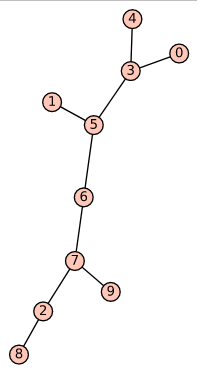
\includegraphics[scale = 0.6]{graf1}\\ 
\scriptsize{\textit{Slika 1: } Naključno drevo na 10 vozliščih.}
\end{center}
Ta seznam, ki ga dobimo v Sage-u kopiramo v Python in dobimo, da je povprečna razdalja med vozlišči 3.4444444444444446, najboljša bližnjica, ki minimizira povprečno razdaljo med vozlišči je med 7 in 0, povprečna razdalja med vozlišči je tedaj 2.0. Če vključimo še eno bližnjico in sicer med 1 in 0, dobimo povprečno razdaljo med vozlišči 1.7777777777777777.
\\[0.5cm]
Poskusimo sedaj na malo večjih drevesih in podatke zapišimo v tabelo:
\\[0.5cm]
\begin{tabular}{ |p{3cm}||p{3cm}|p{3cm}|p{3cm}|  }
 \hline
 \multicolumn{4}{|c|}{Naključna drevesa} \\
 \hline
 Število vozlišč& Povprečna razdalja med vozlišči &Povp. razd. med vozlišči, če vključimo 1 bližnjico&Povp. razd. med vozlišči, če vključimo 2 bližnjici\\
 \hline
 10   & 3.111111111111111    &1.7777777777777777&   1.5555555555555556\\
20&  5.7368421052631575  & 3.526315789473684   &2.526315789473684\\
 30 &6.724137931034483 & 4.931034482758621& 3.5172413793103448\\
 50    &7.551020408163265 & 4.36734693877551& 3.693877551020408\\
 100&  9.04040404040404  & 5.909090909090909&4.393939393939394\\
 \hline
\end{tabular}
\\[0.5cm]
Opazimo, da koda pri drevesih s 100 vozlišči dela že kar počasi, saj mora preveriti vse povezave. Pri iskanju ene bližnjice porabi kakšno minuto, pri dveh pa porabi kar že več kot 2 minuti.
\\[0.5cm]
 Koliko se povprečna razdalja med vozlišči zmanjša, ko vključimo v drevo najboljšo bližnjico?
\newline
Poskusimo narisati v programu R:

\end{document}
